%\section{Outline}
%\input{includes/thesis}
%Given a $m \times n$ system of equations: 
%\section*{Define arithmetic operations ($+, -, \times$) on matrices}
% \section*{Introduction}


\subsubsection*{Objectives}
\begin{itemize}
	\item Define vector (column and row vectors)
	\item Define vector addition and scalar multiplication 
	\item Define linear combination
	\item Provide geometrical interpretation of vectors and linear combinations
\end{itemize}



\subsubsection*{Learning outcomes}
\begin{itemize}
	\item Identify vectors in various dimensions
	\item Perform scalar multiplication and vector addition
	\item Describe linear combinations both geometrically and algebraically
	
    
\end{itemize}





\rule[0.01in]{\textwidth}{0.0025in}
% ---------------------------------------------------- % 


\section{Vectors in $\R^n$}
Vectors result from the need to study and reason about items/objects that have multiple components or variables (e.g., a baby's temperature and weight).  Each variable is associated with a \textbf{dimension}.  In the example above, the baby \textbf{vector} ``lives'' in two-dimensional space since it has associated with it two variables, temperature and weight.  

In general, a two-dimensional  {\color{blue}\textbf{column vector}} is denoted by a bold face lower case letter such as ${\bf v}$, is an \textbf{ordered list}.  Subscripts are used to identify its components: 

\[  {\bf v} = \begin{bmatrix}
	v_1\\v_2
	\end{bmatrix}
\]


The letter ${\bf v}$ was used to emphasize \textbf{v}ector, but other common letters used include ${\bf a, b, c, u, w, x, y, z}$.  For instance,  a three-dimensional vector could be represented as follows (note the use of both square and rounded brackets): 


\[  {\bf x} = \begin{bmatrix}
	x_1\\x_2\\x_3
	\end{bmatrix} = \begin{pmatrix}
	x_1\\x_2\\x_3
	\end{pmatrix}
\]


A \textbf{row vector} is denoted as a horizontal list, 

\[  {\bf v} = (v_1 , v_2, v_3, \dots, v_n) \]

% \begin{bmatrix}
%	v_1 , v_2, v_3, \dots, v_n
%	\end{bmatrix}
 
 %or with parenthesis as in
%\[  
%	(v_1 , v_2, v_3, \dots, v_n)
%\]

\subsubsection*{Notes on Notation}
\begin{enumerate}
	\item Column vectors are preferred over row vectors
	\item Be careful  not to confuse two-dimensional row vectors with points 
	\item Row vectors are use sometimes when typed inline
	\item Square brackets preferred over rounded
	\item When no ambiguity is present, \textbf{bold face} can be replaced by normal typeface
\end{enumerate}



\subsubsection*{Geometrical Interpretation}


 
\begin{figure}[htbp] %  figure placement: here, top, bottom, or page
   \centering

    \includegraphics[scale=0.35]{figures/1_1_1} 
  
   \caption{Geometric interpretation of a vector}
   \label{fig:vector}
\end{figure}
 


\rule[0.01in]{\textwidth}{0.0025in}
% ---------------------------------------------------- % 



%
%%
%%%
%%%% SECTION: Vector Addition
%%%
%%
%
\section{Vector Addition}
% You don't add the components of the vector ($v_1+v_2$), you 

To add vectors, add corresponding vector components. That is, 


\begin{tcolorbox}[colback=yellow!10!,colframe=gray!15!]
\begin{definition}[Vector Addition]
In two-dimensions, if ${\bf x} = \begin{bmatrix}
	x_1 \\ x_2
		\end{bmatrix}$ and ${\bf y} = \begin{bmatrix}
	y_1 \\ y_2
		\end{bmatrix}$, then 
		\[ \]
\[  {\bf x} + {\bf y} = \begin{bmatrix}
	x_1+y_1 \\ x_2 + y_2
		\end{bmatrix} \]
Subtraction is analogous.
  
\end{definition}	 
\end{tcolorbox} 


\begin{example}
	Let  ${\bf x} = \begin{bmatrix}
	3 \\ 1
		\end{bmatrix}$ and ${\bf y} = \begin{bmatrix}
	2 \\ 5
		\end{bmatrix}$, then 
		\[ \]
\[  {\bf x} + {\bf y} = \begin{bmatrix}
	3+2 \\ 1 + 5
		\end{bmatrix} = \begin{bmatrix}
	5 \\ 6
		\end{bmatrix} \]
\end{example}
 
 
 
 

% \subsubsection*{Geometric Interpretation of vector addition}

\begin{figure}
\centering
\begin{subfigure}{.5\textwidth}
  \centering
  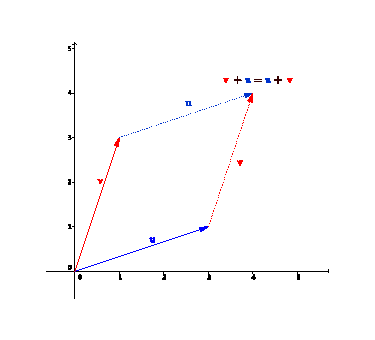
\includegraphics[width=1.1\linewidth]{figures/vec-addition2}
  \caption{}
  \label{fig:sub1}
\end{subfigure}%
\begin{subfigure}{.5\textwidth}
  \centering
  \includegraphics[width=1.0\linewidth]{figures/vec_addition}
  \caption{}
  \label{fig:sub2}
\end{subfigure}
\caption{Geometric Interpretation of vector addition}
\label{fig:test}
\end{figure}





\rule[0.01in]{\textwidth}{0.0025in}
% ---------------------------------------------------- % 


















\section{Scalar Multiplication}
The second operation on vectors is \textbf{scalar multiplication}.  The effect is to ``scale'', (stretch or shrink) the vector.  This is also performed component-wise.


\begin{tcolorbox}[colback=yellow!10!,colframe=gray!15!]
\begin{definition}[Scalar Multiplication]
In two-dimensions, for any $c \in \R$ and ${\bf x} = \begin{bmatrix}
	x_1 \\ x_2
		\end{bmatrix}$, then 
\[  c{\bf x} = \begin{bmatrix}
	cx_1 \\ cx_2
		\end{bmatrix} \]
This notion extends to the $n$-th dimension.  
  
\end{definition}	 
\end{tcolorbox} 

\begin{example}
	Given ${\bf x} = (1,-2)$, then $5{\bf x} = (5, -10)$. 
\end{example}



\rule[0.01in]{\textwidth}{0.0025in}
% ---------------------------------------------------- % 




\begin{example}
	Given ${\bf y} = \begin{bmatrix}
	1 \\ 2 \\ 4
		\end{bmatrix}$, then $3{\bf y} = \begin{bmatrix}
	3 \\ 6 \\ 12
		\end{bmatrix}$. 
\end{example}




%
%%
%%%
%%%% SECTION: Vector Addition
%%%
%%
%
\section{Linear Combinations}

\begin{tcolorbox}[colback=yellow!10!,colframe=gray!15!]
\begin{definition}[Linear Combination\footnote{This is a KEY concept}]
If ${\bf a_1}, {\bf a_2}, \dots, {\bf a_n}$ are $n$ vectors in $\mathbb{R}^m$ and $c_1, c_2, c_3, \dots, c_n \in \mathbb{R}$, then a sum of the form
\[  c_1 {\bf a_1} + c_2 {\bf a_2} + \cdots + c_n {\bf a_n} \]
is called a \textbf{linear combination} of the vectors ${\bf a_1}, {\bf a_2}, \dots, {\bf a_n}$.
  
\end{definition}	 
\end{tcolorbox} 




\begin{example}
	Given ${\bf x} = \begin{bmatrix}
	2 \\ 3 \\ 4
		\end{bmatrix}$ and ${\bf y} = \begin{bmatrix}
	1 \\ 1 \\ -1
		\end{bmatrix}$, then 
		
		
		$
		2\begin{bmatrix}
	2 \\ 3 \\ 4
		\end{bmatrix}  + 3\begin{bmatrix}
	1 \\ 1 \\ -1
		\end{bmatrix} = \begin{bmatrix}
	7 \\ 9 \\ 5
		\end{bmatrix} 
		$ is a linear combination of ${\bf x}$ and ${\bf y}$.
\end{example}




 \rule[0.01in]{\textwidth}{0.0025in}
% ---------------------------------------------------- % 



%\section{Outcome check}
%\begin{questions}
%	\question 
%\end{questions}


%\rule[0.01in]{\textwidth}{0.0025in}
% ---------------------------------------------------- % 





%${\bf v} \to {\bf w}$ is the same as:
%\begin{enumerate}
%\item Find the coordinate vector of ${\bf v}$ with respect to the ordered basis $E$
%\item 
%\end{enumerate}

\subsubsection*{Next time...}
Section 1.2: Lengths and Dot Products

\subsubsection*{Homework}
\textsection1.1: \#2, 3, 4, 26, 27



\subsubsection*{Examples}

These can be done by hand or with GeoGebra.  

\begin{enumerate}

	\item The linear combinations of ${\bf u} = (1,1,0)$ and ${\bf v} = (0 ,1,1)$ fill a plane in $\mathbb{R}^3$.  Describe that plane and fine a vector that is \textit{not} a combination of ${\bf u}$ and ${\bf v}$.  
	
	\textbf{Solution}: {\color{blue} The plane contains all combinations of ${\bf u}$ and ${\bf v}$, namely
	\[  a{\bf u}  +  b {\bf v} = \begin{bmatrix}  a \\ a+b \\ b \end{bmatrix} \]
	
	Since all vectors on the plane have the second component equal to the sum of the first and the third, $(1,2,3)$ is not on the plane.}
	
	  
	\item In the $xy$ plane mark all nine linear combinations of 
	\[ c \begin{bmatrix} 2\\1\end{bmatrix} + d  \begin{bmatrix} 0\\1\end{bmatrix} \;\;\; \text{ with } \;\;\; c=0, 1, 2 \;\;\; \text{ and } \;\;\; d=0, 1, 2 \]
	
	\item If three corners of a parallelogram are $(1,1), (4, 2)$, and $(1,3)$, what are all three of the possible fourth corners?  
	
	
	\item Given ${\bf u}$ and ${\bf v}$ in two-dimensions.  Consider the linear combination 
	\[ c{\bf u} + d {\bf v}   \]  
	
		\begin{enumerate}
			\item Find combinations in which $c+d = 1$.  
			
			\item What are the combinations of 
			\[ c{\bf u} + c {\bf v}?   \]  
			
			
			\item Restrict by $0 \le c,d \le 1$.  What are the combinations $c{\bf u} + d {\bf v}$? 
			
			
			\item Restrict by $0 \le c,d$.  What are the combinations $c{\bf u} + d {\bf v}$?   
			
			\item Generalize to 3-dimensions.
		\end{enumerate}

\end{enumerate}


 

